\section{Theorie}
\label{sec:Theorie}
Dieses Experiment befasst sich mit der Bestimmung der Brechungsindices
von Gasen  und Festkörpern mittels Sagnac-Interferometer.

\subsection{Interferenz}
\subsection{Das Sagnac-Interferometer}
Das Sagnac-Interferometer ist aufgebaut wie in Abbildung \ref{fig:apparat}.
\begin{figure}
    \centering
    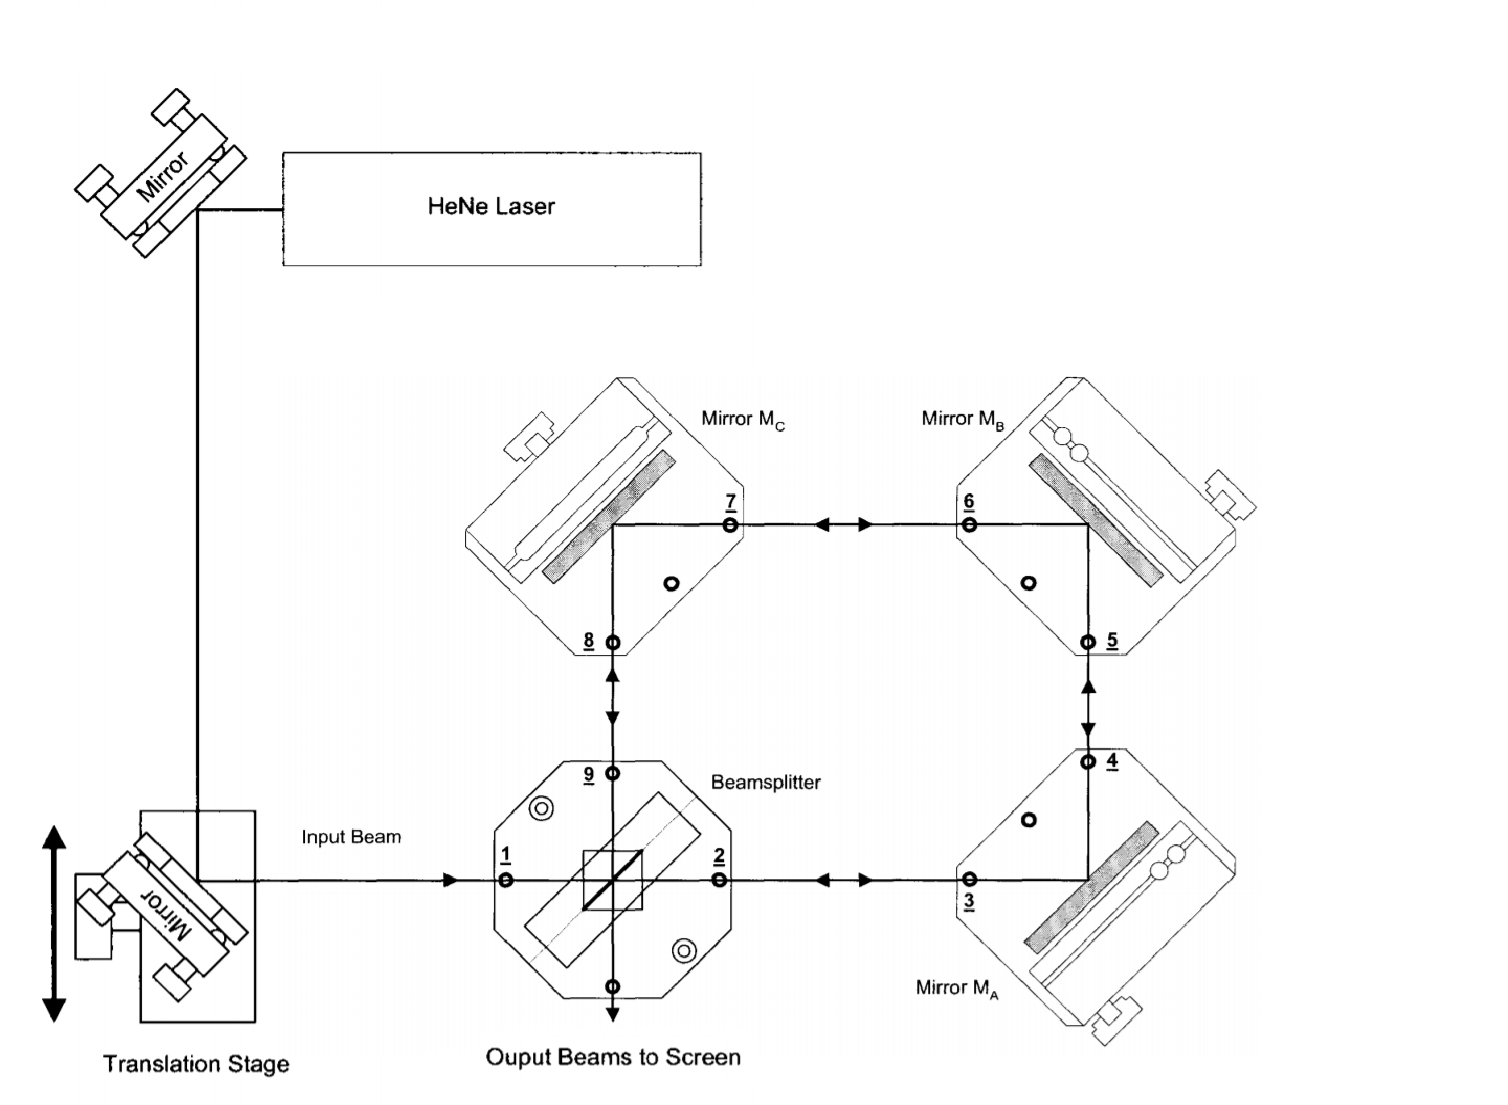
\includegraphics[width=0.7\textwidth]{Apparatur.PNG}
    \caption{Aufbau des Sagnac-Interferometers.\cite{skript}}
    \label{fig:apparat}
\end{figure}
Die Anordnung setzt sich zusammen aus der Quelle, einem HeNe-Laser, zwei
Spiegel zur Ausrichtung des Laserstrahls zum Polarizing-Beam-Splitter-Cube hin.
Zuvor passiert der Laserstrahl einen linearen Polarisationsfilter.
Der PBSC dient zur Aufspaltung des Strahls in Horizntal-und Vertikalkomponente,
dabein passiert die Horizontalkomponente den PBSC und die Vertikalkomponente wird
erfährt einen Richtungsänderung um $90\si{\degree}$. Dies ist in der Abbildung
\ref{fig:pbsc} dargestellt.
\begin{figure}
   \centering
   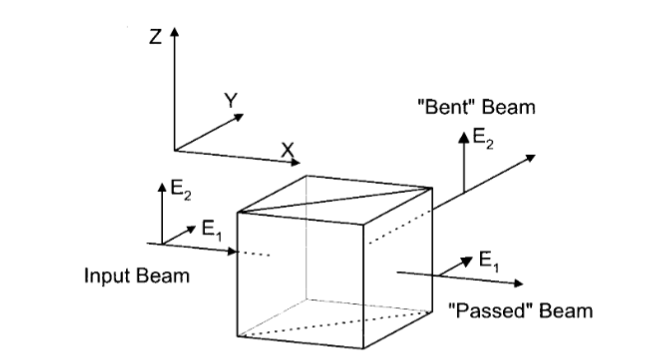
\includegraphics[width=0.7\textwidth]{Pbsc.PNG}
   \caption{Aufaspaltung des Strahls im PBSC.\cite{skript}}
   \label{fig:pbsc}
\end{figure}\\
Drei weitere Spiegel lenken beide Strahle so um, dass diese die gleiche Strecke zurücklegen und wieder auf
den PBSC treffen. Dort werden die Strahlen erneut, nach ihrer polarisation,
umgelenkt und durchgelassen, somit laufen die Strahlen wieder zusammen.
Durch verschieben der Translation Stage können die zwei Strahlen räumlich separiert
werden und somit unterschiedliche Materialien durchqueren.
%Bei der ersten Messung werden zwei Glasplättchen, die auf einer Rotationsachse
%befestigt sind, unterschiedlicher
%Ausrichtung in die beiden Strahlengänge positioniert, zu sehen in der Abbildung
\ref{fig:glasplattchen}.


\subsection{Brechungsindex von Gasen}
Für die Bestimmung vom Brechungsindex von Gasen wird eine Gaszelle
der Länge $L$ genutzt. Einer der Strahlen passiert dabei die Gaszelle.
Ändert sich der Druck innerhalb der Gaszelle, so ändert sich auch
der Brechungsindex des Gases. Dies erzeugt eine Phasenverschiebung:
\begin{align}
  \Delta\phi=\frac{2\pi}{\lambda_\mathrm{vac}}(n-1)L
\end{align}
Durch diese Phasenverschiebung entstehen Interferenzerscheinungen.
Die Interferenzmaxima $M$ sind in folgender Beziehung abhängig
vom Brechungsindex $n$:
\begin{align}
  M=\frac{n-1}{\lambda_\mathrm{vac}}L
\end{align}
\subsection{Brechungsindex von Festkörpern}
